\documentclass[11pt]{article}
\usepackage[utf8]{inputenc}
\usepackage[T1]{fontenc}
\usepackage{fixltx2e}
\usepackage{graphicx}
\usepackage{longtable}
\usepackage{float}
\usepackage{wrapfig}
\usepackage{soul}
\usepackage{textcomp}
\usepackage{marvosym}
\usepackage{wasysym}
\usepackage{latexsym}
\usepackage{amssymb}
\usepackage{hyperref}
\tolerance=1000
\usepackage{fullpage}
\providecommand{\alert}[1]{\textbf{#1}}

\title{Report on Doppler Shift Experiment}
\author{Craig Roy}
\date{\today}
\hypersetup{
  pdfkeywords={},
  pdfsubject={},
  pdfcreator={Emacs Org-mode version 7.9.3f}}

\begin{document}

\maketitle


\section*{Description}
\label{sec-1}

This experiment consists of a spectrometer observing an exoplanet. The
relatively stationary observer will see that the absorption spectra
for the exoplanet differ when it is moving towards and away from them.
\section*{How to use it}
\label{sec-2}

The angular velocity of the planet is set using the slider at the
bottom of the window. The absorption spectra for the exoplanet
are shown above the slider. When the slider is moved so the angular
velocity isn't 0, the absorption spectra will begin to shift.

There is also a plot of the emission spectra for the exoplanet which
can be opened by checking the ``Show emission plot'' checkbox at the
bottom of the window.
\section*{How it works}
\label{sec-3}
\subsection*{Variables}
\label{sec-3-1}

\begin{itemize}
\item \emph{a} is the angle of rotation of the exoplanet from the northern position.
\item \emph{r, r2} are the radius of the path travelled by the exoplanet and
  the radius of the path travelled by the star it orbits respectively.
\item \emph{x, y} are the x and y coordinates of the exoplanet. These
  coordinates are determined from the angle of the planet, \emph{a}, and
  the radius of the path travelled by the exoplanet, \emph{r}.
\item \emph{vx, vy} are the velocity of the exoplanet in the x and y axes
  respectively. They are also calculated from the angle of the planet,
  as well as the angular velocity of the system, \emph{omega}.
\item \emph{t} is the time variable for the evolution of the system.
\item \emph{off} is the offset added to the position of the star-planet
  system to move it to the right of the spectrometer image.
\item \emph{segment} is the two-dimensional array of coordinates for the absorption lines.
\item \emph{posRef} is the array of positions of the absorption lines before
  the Doppler shift is applied.
\item \emph{offset} is the amount which the position of the absorption lines should be offset by the Doppler shift caused by the motion of the planet.
\item \emph{x2, y2} are the x and y positions of the star.
\item \emph{omega} is the angular velocity of both the exoplanet and the star.
\end{itemize}
\subsubsection*{Plotting Variables}
\label{sec-3-1-1}

\begin{itemize}
\item \emph{xPoints, yPoints} are the arrays of coordinates for the points to plot on the emission spectrum plot.
\item \emph{waveOffset} is the amount which the wavelengths of the emission lines should be shifted due to the Doppler effect.
\item \emph{showPlot} is the variable behind the ``Show Emission Plot'' checkbox.
\item \emph{lamRef} is the array of x-coordinates for the points on the graph not considering the Doppler shift.
\end{itemize}
\subsection*{Initialisation}
\label{sec-3-2}

In the initialisation, an array of four random wavelengths between
400nm and 700nm are randomly generated and used to populate the
arrays, \emph{xPoints} and \emph{lamRef}. They are given a corresponding value
in \emph{yPoints} between 0 and 0.2. Then, ten points from the array are
randomly chosen as the absorption spectra and these points are given
corresponding y-coordinates with values between 0.2 and 1. These wavelengths are then scaled down to values
between -1 and 1 for use plotting the absorption lines on the spectrum
of visible light. These are used to populate the two-dimensional
array, \emph{segment}, where the second dimension is the y-coordinate, -1
in order to place the lines at the bottom of the screen.
\subsection*{Evolution}
\label{sec-3-3}
\subsubsection*{Evol Page}
\label{sec-3-3-1}

The first evolution page introduces the relationship between the angle of rotation, \emph{a}, and the angular velocity, \emph{omega}.
\subsubsection*{Spectra}
\label{sec-3-3-2}

For each step of the evolution of the system, this page sets the positions and the points of the spectral lines equal to their reference values plus the appropriate Doppler shift.
\subsection*{Fixed relations}
\label{sec-3-4}

The fixed relations page contains relationships generating x and y coordinates and velocities from the angle of the planet and star.
It also generates the offset for the positions and wavelengths of the absorption spectra based on the magnitude of the velocity in the x-axis.
\subsection*{Custom}
\label{sec-3-5}

\begin{itemize}
\item \emph{positionToWavelength} takes a position on the spectrum between -1 and 1 and converts it to the equivalent wavelength in nanometers (between 400nm and 700nm) for plotting on the graph.
\item \emph{wavelengthToPosition} does the opposite of the \emph{positionToWavelength} method.
\item \emph{randomPosition} generates a random value between -1 and 1 to be used as a position for an absorption line.
\end{itemize}
\subsection*{UI}
\label{sec-3-6}
\subsubsection*{Frames}
\label{sec-3-6-1}

The UI of this experiment consists of two windows: the simulation
window and the plotting window. The plotting window is hidden by
default and is opened with the ``Show emission plot'' checkbox at the
bottom of the simulation window.

The simulation window contains the model exoplanet orbiting a star,
showing their paths. It also shows the absorption lines for the
exoplanet plotted on the spectrum of visible light. It has a slider at
the bottom to change the angular velocity of the planet, as well as
the play/pause button, the reset button and the checkbox to show the
emission spectrum plot.
\subsubsection*{Images}
\label{sec-3-6-2}

This simulation makes use of two images. A drawing of a telescope, to
act as a mock spectrometer, and a picture of the spectrum of visible
light, to be the background for the spectral lines. Both of these
images are freely licensed.

\begin{figure}[htb]
\centering
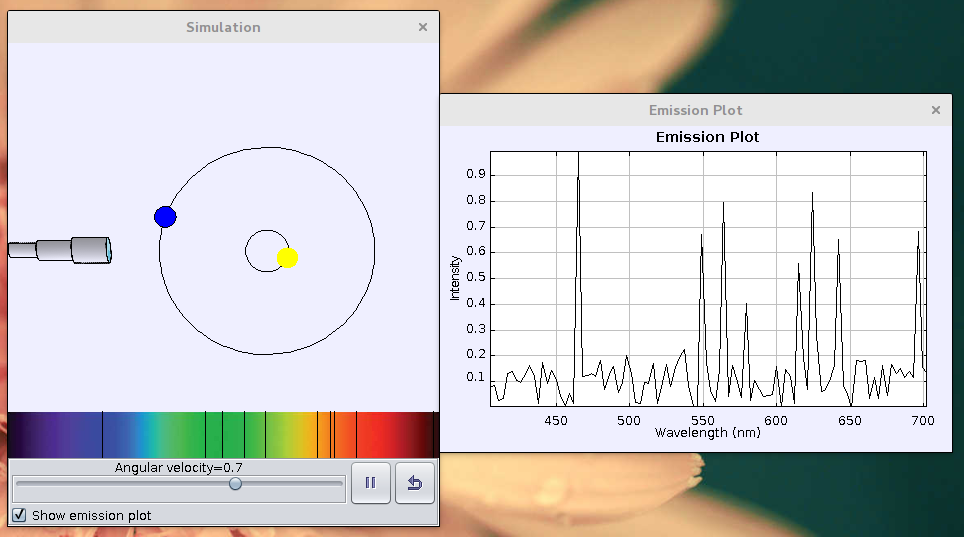
\includegraphics[width=.9\linewidth]{./dopplerUI.png}
\caption{UI of the Doppler shift experiment}
\end{figure}

\end{document}
